\documentclass[a4paper, 12pt]{report}

\usepackage[dvipsnames]{xcolor}

%%%%%%%%%%%%%%%%%
% Set Variables %
%%%%%%%%%%%%%%%%%

\def\useItalian{0}  % 1 = Italian, 0 = English

\def\courseName{Network Algorithms}

\def\coursePrerequisites{
    \begin{itemize}
        \item Progettazione di Algorithmi
    \end{itemize}
}

\def\book{TODO}

% \def\authorName{Simone Bianco}
% \def\email{bianco.simone@outlook.it}
% \def\github{https://github.com/Exyss/university-notes}
% \def\linkedin{https://www.linkedin.com/in/simone-bianco}

\def\authorName{Alessio Bandiera}
\def\email{alessio.bandiera02@gmail.com}
\def\github{https://github.com/aflaag-notes}
\def\linkedin{https://www.linkedin.com/in/alessio-bandiera-a53767223}

% Do not change

%%%%%%%%%%%%
% Packages %
%%%%%%%%%%%%

\usepackage{../../packages/Nyx/nyx-packages}
\usepackage{../../packages/Nyx/nyx-styles}
\usepackage{../../packages/Nyx/nyx-frames}
\usepackage{../../packages/Nyx/nyx-macros}
\usepackage{../../packages/Nyx/nyx-title}
\usepackage{../../packages/Nyx/nyx-intro}

%%%%%%%%%%%%%%
% Title-page %
%%%%%%%%%%%%%%

\logo{../../packages/Nyx/logo.png}

\ifx\useItalian0
    \institute{\curlyquotes{\hspace{0.25mm}Sapienza} Università di Roma}
    \faculty{Ingegneria dell'Informazione,\\Informatica e Statistica}
    \department{Dipartimento di Informatica}
    \subtitle{Appunti integrati con il libro \book}
    \author{\textit{Autore}\\\authorName}
\else
    \institute{\curlyquotes{\hspace{0.25mm}Sapienza} University of Rome}
    \faculty{Faculty of Information Engineering,\\Informatics and Statistics}
    \department{Department of Computer Science}
    \subtitle{Lecture notes integrated with the book \book}
    \author{\textit{Author}\\\authorName}
\fi

\title{\courseName}
\date{\today}

% \supervisor{Linus \textsc{Torvalds}}
% \context{Well, I was bored\ldots}

\addbibresource{./references.bib}

%%%%%%%%%%%%
% Document %
%%%%%%%%%%%%

\begin{document}
    \maketitle

    % The following style changes are valid only inside this scope 
    {
        \hypersetup{allcolors=black}
        \fancypagestyle{plain}{%
        \fancyhead{}        % clear all header fields
        \fancyfoot{}        % clear all header fields
        \fancyfoot[C]{\thepage}
        \renewcommand{\headrulewidth}{0pt}
        \renewcommand{\footrulewidth}{0pt}}

        \romantableofcontents
    }

    \introduction

    %%%%%%%%%%%%%%%%%%%%%

    \chapter{TODO}

    \section{Introduction on graphs}

    In many network applications, graphs are used as a natural model. In other applications, the graph model may be less obvious, but appears to be anyway very useful. Graph algorithms are useful instruments to solve important and living problems. We will see a number of advanced techniques for efficient algorithm design to solve problems from networks and graphs. 

    \begin{frameddefn}{Graph}
        A \textbf{graph} is a mathematical structure $G = (V,E)$ made of a set $V$ called the \textit{vertex set} (or \textit{node set}), and a set $E \subseteq V \times V$ called \textit{edge set}.
    \end{frameddefn}

    Graphs are usually represented through circles and lines, were each line between two vertices $u,v$ represents the edge $(u,v)$. We will assume to be working with \textit{simple graphs}, a type of graph that doesn't allow loop edges, i.e. edges from a node to itself, or a multiple number of edges between two vertices.  
   

    The edges of a graph can also be \textit{directed} or \textit{undirected}. In the former, the two edges $(u,v)$ and $(v,u)$ are considered two distinct edges while in the latter they are considered as the same edge. A directed graph is usually also referred to as \textbf{digraph}. 
    
    \begin{figure}[H]
        \centering

        \begin{tabular}{ccc}
            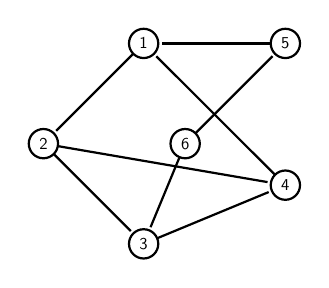
\begin{tikzpicture}[-,>=stealth,shorten >=1pt,auto,node distance=3cm,thick,main node/.style={scale=0.6,circle,draw,font=\sffamily\normalsize}]
                \node[main node] (1) {1};
                \node[main node] (2) [below left of=1] {2};
                \node[main node] (3) [below right of=2] {3};
                \node[main node] (6) [right of=2] {6};
                \node[main node] (5) [above right of=6] {5};
                \node[main node] (4) [below of=5] {4};
    
                \path[every node/.style={font=\sffamily\small}]
                    (1) edge (2)
                    (2) edge (3)
                    (2) edge (4)
                    (3) edge (4)
                    (4) edge (1)
                    (5) edge (1)
                    (6) edge (3)
                    (6) edge (5)
                    ;
            \end{tikzpicture}

            &\qquad\qquad&

            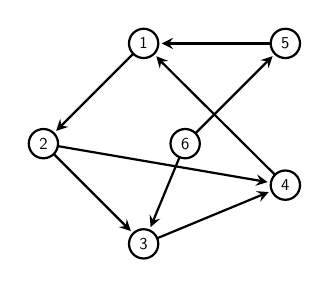
\begin{tikzpicture}[->,>=stealth,shorten >=1pt,auto,node distance=3cm,thick,main node/.style={scale=0.6,circle,draw,font=\sffamily\normalsize}]
                \node[main node] (1) {1};
                \node[main node] (2) [below left of=1] {2};
                \node[main node] (3) [below right of=2] {3};
                \node[main node] (6) [right of=2] {6};
                \node[main node] (5) [above right of=6] {5};
                \node[main node] (4) [below of=5] {4};
    
                \path[every node/.style={font=\sffamily\small}]
                    (1) edge (2)
                    (2) edge (3)
                    (2) edge (4)
                    (3) edge (4)
                    (4) edge (1)
                    (5) edge (1)
                    (6) edge (3)
                    (6) edge (5)
                    ;
            \end{tikzpicture}
        \end{tabular}

        \caption{On the left: a simple graph. On the right: a simple digraph}
    \end{figure}

    Graphs were born in 1736, when Euler used them formalize and solve the famous \textit{Seven Bridges of Königsberg} problem: is there a way to walk through all the bridges of the town and end up on the starting point? 

    \begin{figure}[H]
        \centering

        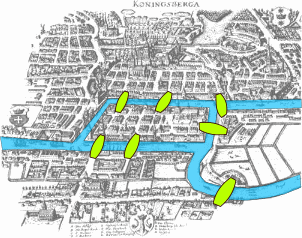
\includegraphics[scale=0.6]{../assets/Konigsberg_bridges.png}
        \caption{The city of Königsberg and its seven bridges}
    \end{figure}

    To solve the problem, Euler represented the problem as the following \textit{multi-graph}, i.e. a non-simple graph that allows multiple edges between two vertices. Euler proved that the answer to the question is negative: a walk that passes through all the edges of such graph while also returning to the starting node cannot exist.

    \begin{figure}[H]
        \centering
        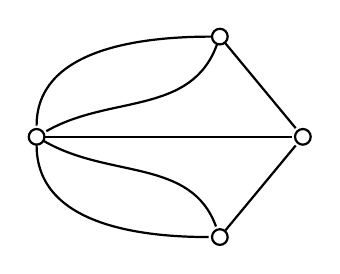
\begin{tikzpicture}[-,>=stealth,shorten >=1pt,auto,node distance=3cm,thick,main node/.style={scale=0.6,circle,draw,font=\sffamily\normalsize}]
            \node[main node] (1) {};
            \node[main node] (2) [below left of=1, xshift = -50] {};
            \node[main node] (3) [below right of=2, xshift = 50] {};
            \node[main node] (4) [right of=2, xshift = 75] {};

            \path[every node/.style={font=\sffamily\small}]
                (1) edge [out=180, in=90] (2)
                (1) edge [out=-110, in=30] (2)
                (2) edge [out=270, in=180] (3)
                (2) edge [out=-30, in=110] (3)
                (2) edge (4)
                (1) edge (4)
                (3) edge (4)
                ;
        \end{tikzpicture}

        \caption{The multi-graph representing the Seven Bridges of Königsberg problem}
    \end{figure}

    In general, a \textbf{walk} on a graph $G$ is given by a sequence of nodes $v_1, \ldots, v_k$ such that $(v_i, v_{i+1}) \in E(G)$. A \textbf{path} is walk whose vertices are all distinct. As we'll see in the following sections, walks and paths are the basis of graph theory.

    \newpage

    \section{The routing problem}

    When packets are sent from a computer to another through a network, each computer has to route data on a path passing through intermediate computers. This problem is usually referred to as the \textbf{routing problem}.
    
    By modelling the network as a graph whose vertices correspond to the computers and its edges correspond to the links between them, such problem is reduced to the concept of a path from an initial node to an arrival node.

    Based on the required conditions, the routing reduces to a specific type of path problem:
    \begin{enumerate}
        \item In \textbf{non-adaptive routing}, the routing algorithm must minimize the number of intermediate computers on the route. This problem reduces to the \textit{shortest path problem}, i.e. finding the path that passes through the lowest amount of edges from node $s$ to node $t$. This type of routing gives good results with consistent topology and traffic conditions, but performs poorly in case of congestion. 
        \item In \textbf{adaptive routing}, the routing algorithm must take into account the traffic conditions: if a route is congested, we want to avoid it in. This problem reduces to the \textit{least cost path problem}, i.e. finding the path with the least cost from node $d$ to node $t$. This type of routing gives good results with high network workload, but routes must be computed frequently in order to perform well.
        \item In \textbf{fault-sensitive routing}, the routing algorithm must consider the possibility of a link failing: we want the route with the highest probability of working. 
    \end{enumerate}


    Each of these problems can be modeled as a graph. In particular, adaptive routing and fault-sensitive routing need an additional \textit{weight function} $w : E(G) \to \R$ such that $w(e)$ represents the weight of an edge $e \in E(G)$. The \textbf{weight (or cost) of a path} $P$, written as $w(P)$, is the sum of the edges that compose it.

    \begin{example}[Weighted graphs]
        The following is an example of a graph with weights on the edges.

        \begin{figure}[H]
            \centering
            \begin{tikzpicture}[-,>=stealth',shorten >=1pt,auto,node distance=3cm,thick,main node/.style={scale=0.6,circle,draw,font=\sffamily\normalsize}]
                \node[main node] (1) {1};
                \node[main node] (2) [above of=1] {2};
                \node[main node] (3) [right of=2] {3};
                \node[main node] (4) [below of=3] {4};

                \path[every node/.style={font=\sffamily\small}]
                    (1) edge node {1} (2)
                    (2) edge node {2} (3)
                    (3) edge node {5} (4)
                    (4) edge node {10} (1)
                    (1) edge node {6} (3)
                    ;
            \end{tikzpicture}
            \caption{An indirected weighted graph.}
        \end{figure}

        For instance, the path $1, 2, 3, 4$ has weight $1 + 2 + 5 = 8$.
    \end{example}
    
    The weight measure varies based on the context. In adaptive routing the traffic acts as the weight, while in fault-sensitive routing the probability acts as the weight. In particular, let $p(u,v)$ be the probability that an edge $(u,v) \in E(G)$ doesn't fail. Under the not-so-realistic assumption that edge failures occur independently of each other, we get that the probability that a path $P = v_1, \ldots, v_k$ doesn't fail is given by $p(v_1, v_2) \cdot \ldots \cdot p(v_{k-1}, v_k)$.
    
    By setting each weight $w(u,v)$ equal to $-\log(p(u,v))$, we get that the product $p(v_1, v_2) \cdot \ldots p(v_{k-1}, v_k)$ reaches its maximum when the sum $w(v_1, v_2) + \ldots + w(v_{k-1}, v_k)$ reaches its minimum. Through this weight function, fault-sensitive routing is also reduces to the least cost path problem.

    Similarly, the shortest path problem can also be reduced to the least cost path problem by setting $w(u,v)$ equal to 1 for each edge. One problem to rule them all!

    \begin{frameddefn}{Distance}
        Let $G = (V,E)$ be a graph. Given two nodes $u,v \in V(G)$, the \textbf{distance} between $u$ and $v$, written as $\dist(u,v)$, is the minimum weight of all the paths $u \to v$ of $G$.
    \end{frameddefn}

    On digraphs the concept of distance is non-symmetrical: the distance $\dist(u,v)$ may be different from the distance $\dist(v,u)$. Moreover, when there is no path $u \to v$, we assume that $\dist(u,v) = +\infty$.

    \section{TODO}
    
    \subsection{Classical solutions}
    
    \begin{algorithm}[H]
        \caption{
            \textit{Bellman-Ford}: TODO
        }

        \label{alg:bellman_ford}
        \begin{algorithmic}[1]
            \Function{bellmanFord}{$G$}
                \State TODO
            \EndFunction
        \end{algorithmic}
    \end{algorithm}

    \begin{algorithm}[H]
        \caption{
            \textit{Dijkstra}: TODO
        }

        \label{alg:dijkstra}
        \begin{algorithmic}[1]
            \Function{dijkstra}{$G$}
                \State TODO
            \EndFunction
        \end{algorithmic}
    \end{algorithm}

    \begin{framedalgo}{Floyd-Warshall}
        Given a directed graph $G$, and an unconstrained weight function $w$ for the edges, the algorithms returns a matrix \texttt{dist} such that $\arraytt{dist}{u}{v}$ is the weight of the least-cost path from $u$ to $v$. \\

        \hrule

        \quad
        \label{alg:floyd_warshall}
        \begin{algorithmic}[1]
            \Function{floydWarshall}{$G$, $w$}
                \State Let $\texttt{dist[}n\texttt{][}n\texttt{]}$ be an $n \times n$ matrix, initialized with every cell at $+ \infty$
                \For{$u \in V(G)$}
                    \State $\arraytt{dist}{u}{u} = 0$
                \EndFor
                \For{$(u, v) \in E(G)$}
                    \State $\arraytt{dist}{u}{v} = w(u, v)$
                \EndFor
                \For{$k \in V(G)$}
                    \For{$u \in V(G)$}
                        \For{$v \in V(G)$}
                            \State $\arraytt{dist}{u}{v} = \min \rbk{\arraytt{dist}{u}{v}, \arraytt{dist}{u}{k} + \arraytt{dist}{k}{v}}$
                        \EndFor
                    \EndFor
                \EndFor
            \EndFunction
        \end{algorithmic}
    \end{framedalgo}
   
    \idea{
        The core concept of the algorithm is to construct a matrix using a \href{https://en.wikipedia.org/wiki/Dynamic_programming}{dynamic programming} approach, that evaluates all possible paths between every pair of vertices. Specifically, to determine the shortest path from a vertex $u$ to a vertex $v$, the algorithm considers two options: either traveling directly from $u$ to $v$, or passing through an intermediate vertex $k$, potentially improving the path.
    }

    \cost{
        The \texttt{for} loop in line 3 has cost $\Theta(n)$, the \texttt{for} loop in line 6 has cost $\Theta(m) = \Theta(n^2)$ and the cost of the triple nested \texttt{for} loop is simply $\Theta(n^3)$. Therefore, the cost of the algorithm is $$\Theta(n) + \Theta(n^2) + \Theta(n^3) = \Theta(n^3)$$
    }

    \section{Interconnection topologies}

    Up to this point, the routing problem has considered the network as a graph where \tbf{the structure is not known to the nodes}, and can change over time due to factors like \tit{faults} and \tit{variable traffic}. However, when the network represents an \tbf{interconnection topology}, such as one connecting processors, the structure of the network is known and remains fixed. This characteristic can be leveraged in the packet-routing algorithms.

    While the fixed nature of the network topology can be used to develop more efficient routing strategies, efficiency becomes a critical concern in interconnection topologies. As a result, solutions with stronger properties than basic shortest-path algorithms are required.

    There are many types of routing models. In this notes, the focus will be on the \href{https://en.wikipedia.org/wiki/Store_and_forward}{store-and-forward} model:

    \begin{itemize}
        \item aata is divided into \tit{discrete packets};
        \item each packet contains \tit{control information} (such as source, destination, and sequence data) and is treated as an independent unit that is forwarded from node to node through the network;
        \item packets may be temporarily stored in \tbf{buffer queues} at intermediate nodes if necessary, due to link congestion or busy channels;
        \item each node makes a \tbf{local routing decision} based on the packet's destination address and the chosen routing algorithm;
        \item during each step of the routing process, \tbf{a single packet can cross each edge};
        \item additionally, mechanisms for error detection and recovery may be employed to ensure reliable packet delivery, and flow control and congestion management may be applied to optimize network performance.
    \end{itemize}

    \subsection{Butterfly networks}

    \begin{frameddefn}{Butterfly network}
        Let $n$ be an integer, and let $N := 2^n$; an \tbf{$n$-bufferfly network} is a \tit{layered graph} defined as follows:

        \begin{itemize}
            \item there are $n + 1$ layers of $N$ nodes each, for a total of $N(n + 1)$ nodes;
            \item each node is labeled with a pair $(w, i)$, where $i$ is the \tit{layer of the node}, and $w$ is an $n$-bit binary number that denotes the \tit{row of the node};
            \item there are $2Nn = 2 \cdot 2^n \cdot n = n2^{n + 1}$ edges;
            \item two nodes $(w, i)$ and $(w', i')$ are linked by an edge if and only if $i' = i + 1$ and either $w = w'$ (which is a \tit{straight edge}) or $w$ and $w'$ differ in only the $i$-th bit (which is a \tit{cross edge}).
        \end{itemize}
    \end{frameddefn}

    \begin{example}[Butterfly network]
        The following figure shows an example of a butterfly network.

        \centeredimage[A butterfly network.]{0.35}{../assets/butterfly.png}
    \end{example}

    Note that the nodes of a butterfly network can be \tbf{rearranged} to form a mirror image of the original network.

    Butterfly networks have a \tbf{recursive structure}, which is highlighted in the following figure. Specifically, one $n$-dimensional butterfly contains two $(n - 1)$-dimensional butterfly networks as subgraphs.

    \centeredimage[The recursive structure of butterfly networks.]{0.3}{../assets/butterfly_recursive.png}

    Through the recursive structure of the butterfly network it can be easily shown, by structural induction, that each node of the network has degree 4, except for the ones in the first and last layer. Therefore, to perform the routing of the packets on a butterfly network, its nodes are \tbf{crossbar switches}, which have two input and two output ports and can operate in two states, namely \tit{cross} and \tit{bar} (shown below, respectively).

    \centeredimage[A butterfly network node.]{0.25}{../assets/butterfly_nodes.png}

    Usually, $4N$ additional nodes are typically added ($2N$ for the input, and $2N$ for the output) such that $\deg(u) = 4$ for each $u \in V(G)$ --- these nodes will not be considered in the networks analyzed in this notes.

    \centeredimage[An extended butterfly network.]{0.25}{../assets/butterfly_extended.png}

    As a result, a butterfly network can be viewed as a \tit{switching network} that connects $2N$ input units to $2N$ ouptut units, through a layered structure divided into $\log N +1 = \log 2^n +1 = n + 1$ layers, each consisting of $N$ nodes.

    The topology of the butterfly network can be leveraged as stated in the following proposition.

    \begin{framedprop}[label={prop:greedy_path}]{Greedy path}
        Given a pair of rows $w$ and $w'$, there exists a \tit{unique path of length $n$}, called \tbf{greedy path}, from node $(w, 0)$ to node $(w', n)$. This path passes through each layer exactly once, and it can be found through the following procedure:

        \begin{algorithmic}[1]
            \Function{greedyPath}{$w$, $w'$}
                \For{$i \in [1, n]$}
                    \If{$w_i == w'_i$}
                        \State Traverse a \tit{straight edge}
                    \Else
                        \State Traverse a \tit{cross edge}
                    \EndIf
                \EndFor
            \EndFunction
        \end{algorithmic}
    \end{framedprop}

    Packet-routing performed on a butterfly network can pose some challenges. Assume that each node $(u, 0)$ in the network on layer 0 of the butterfly contains a packet, which is destined for node $(\pi(u), n)$ in layer $n$ --- there are $n + 1$ layers, ranging in $[0, n]$ --- where $$\func{\pi}{[1, N]}{[1, N]}$$ describes the permutation of the packet destinations. In a \tbf{greedy routing algorithm}, each packet follows its \tit{greedy path}, meaning that at each intermediate layer, it makes progress toward its final destination by choosing the edges to cross through the algorithm described in \cref{prop:greedy_path}.

    When routing only a \tit{single packet}, the greedy algorithm works efficiently, since there are no conflicts or competing resources along the path. However, when \tit{multiple packets} are routed in parallel, conflicts can arise, especially when multiple packets attempt to traverse the same edge or node simultaneousl. n fact, \tit{multiple greedy paths} may intersect at the same node or edge, and since only one packet can traverse a given edge at any moment, the other packets must be \tbf{delayed} until the edge becomes available. As a result, the butterfly network cannot route every permutation without delays, making it a \tbf{blocking network}.

    For simplicity, assume that $n$ is odd (though similar results hold for even values of $n$), and consider the following edge $$e :=  \rbk{ \rbk{0 \ldots 0, \frac{n-1}{2}},  \rbk{ 0 \ldots 0,\frac{n+1}{2} } }$$ Note that $e$'s endpoints are the roots of two complete binary trees, which have $2^{\frac{n -1}{2}}$ and $2^{\frac{n + 1}{2}}$ nodes respectively.

    \centeredimage{0.3}{../assets/butterfly_trees.png}

    In the worst case, $\pi$ can be such that \tit{each greedy path starting from a leaf on the left tree and ending on a leaf on the right tree traverses $e$}. Note that the number of such paths is precisely the number of leafs of the left complete binary tree, namely $2^\frac{n- 1}{2} = \sqrt{\frac{N}{2}}$. Therefore, in the worst case $\sqrt{\frac{N}{2}}$ packets may need to traverse $e$, which means that one of them may be delayed by $\sqrt{\frac{N}{2}} - 1$ steps. Since it takes $n = \log N$ steps to traverse the whole network, the greedy algorithm can take up to $$\sqrt{\dfrac{N}{2}} -1 + \log N$$ steps to route a permutation.

    The following theorem generalizes this result.

    \begin{framedthm}{Butterfly routing}
        Given any routing problem on a $n$-dimensional butterfly network, for which at most one packet starts at each $0$-th layer node, and at most one packet is destined for each $n$-th layer node, the \tit{greedy algorithm} will route all the packets to their destination in $O (\sqrt N)$ steps.
    \end{framedthm}

    \begin{proof}
        For simplicity, assume that $n$ is odd (though similar results can be proven for even values of $n$). Given $0 < i \le n$, let $e$ be any edge in the $i$-th layer, and let $n_i$ be the number of greedy paths traversing $e$.

        The number of greedy paths in the first half of the butterfly is bounded by the number of leaves of the left complete binary tree, namely $n_i \le 2^{i - 1}$. Analogously, on the second half of the butterfly, $n_i$ is bounded by the number of leaves of the right complete binary tree, therefore $n_i \le 2^{n - i}$. Note that both this results hold because $n$ is odd.

        Note that any packet that need to cross $e$ can be delayed by \tit{at most} the other $n_i - 1$ packets. Therefore, recalling that $\displaystyle \sum_{j = 0}^k {2^j} = 2^{k + 1} - 1$, as a packet traverses layers 1 through $n$, the total delay it can encounter is at most

        \begin{equation*}
            \begin{split}
                \sum_{i = 1}^n {(n_i -1)} &= \sum_{i = 1}^\frac{n + 1}{2} {(n_1 - 1)} + \sum_{i = \frac{n + 1}{2} + 1}^n(n_i - 1) \\
                                          &\le \sum_{i = 1}^\frac{n + 1}{2} {\rbk{2^{i - 1} - 1}} + \sum_{i = \frac{n + 3}{2}}^n {\rbk{2^{n - i} - 1}} \\
                                          &= \sum_{j = 0}^{\frac{n + 1}{2} - 1}{\rbk{2^j - 1}} + \sum_{j = 0}^{\frac{n - 3}{2}} {\rbk{2^j - 1}} \\
                                          &=\sum_{j = 0}^{\frac{n + 1}{2} - 1}{2^j} + \sum_{j = 0}^{\frac{n - 3}{2}} {2^j} - n \\
                                          &=2^{\frac{n + 1}{2}} - 1 + 2^{\frac{n - 1}{2}} - 1 - n \\
                                            &\le O(\sqrt N) - n \\
                                            &\le O(\sqrt N)
            \end{split}
        \end{equation*}
    \end{proof}

    Although such a greedy routing algorithm performs poorly in the worst case, it is \tbf{highly effective in practice}. In fact, for many practical classes of permutations, the greedy algorithm runs in $n$ steps, which is optimal, and for most permutations the algorithm runs in $n + o(n)$ steps. Consequently, the greedy algorithm is widely used in real-world applications.

    \subsection{Beneš networks}

    As shown in the previous section, the \tit{butterfly network} can present efficiency problems due to packet delays caused by congestion when multiple packets are routed simultaneously. One way to \tit{avoid routing delays} is by using a \tbf{non-blocking topology}.

    \begin{frameddefn}{Beneš network}
        An \tbf{$n$-dimensional Beneš network} is a network constructed by placing \tit{two $n$-dimensional butterfly networks back-to-back}.
    \end{frameddefn}

    \begin{example}[Beneš network]
        The following is an example of a Beneš network.

        \centeredimage[A Beneš network.]{0.2}{../assets/benes.png}
    \end{example}

    Note that an $n$-dimensional Beneš network has $$2(n + 1) - 1 = 2n + 2 - 1 = 2n + 1$$ layers, because the two $n$-dimensional butterfly network --- which describe the first and last $n + 1$ layers --- have an \tit{overlapping layer}.

    Consider the following property.

    \begin{frameddefn}{Rearrangeability}
        A network with $N$ inputs and $N$ outputs is said to be \tbf{rearrangeable} if, for any one-to-one mapping $\pi$ of the inputs to the outputs, the mapping can be realized using exclusively \tit{edge-disjoint paths}.
    \end{frameddefn}
    
    As for the case of the butterfly network, two inputs and two outputs are typically connected at both the beginning and end of the Beneš network, ensuring that each node has a degree of 4. Therefore, this type of Beneš network has $2N = 2 \cdot 2^n = 2^{n + 1}$ inputs linked to the $0$-th layer, and $2^{n + 1}$ layers linked to the $2n$-th layer.

    However, in the case of the Beneš network, the following theorem will establish an important result that leverages these additional inputs and outputs.

    \begin{framedthm}{Rearrangeability of the Beneš network}
        Any $n$-dimensional Beneš network is rearrangeable.
    \end{framedthm}

    \proofind{
        The proof proceeds by induction on $n$.
    }{
        When $n = 0$, the Beneš consists of a single node, the theorem is vacuously true, because there are no edges on the network.
    }{
        Given any one-to-one mapping $\pi$ of the $2^n$ inputs and outputs of a $(n - 1)$-dimensional Beneš network, there exists \tit{a set of edge-disjoint paths} from the inputs to the outputs, connecting each input $i$ to output $\pi(i)$, for each $1 \le i \le 2^{n}$.
    }{
        Consider an $n$-dimensional Beneš network, with $2^{n + 1}$ inputs and outputs; note that its middle $2n - 1$ layers describe two $(n - 1)$-dimensionl Beneš networks, as shown in figure.

        \centeredimage[Subnetworks of a Beneš network.]{0.2}{../assets/benes_subnetworks.png}


        Note that each \tit{starting node} --- those in layer 0 --- has degree 4, and 2 of the links connect each starting node to the inputs, external to the Beneš network. Therefore, by definition of the Beneš network, the remaining two edges must connect each starting node with the two separate $(n - 1)$-dimensional Beneš networks. Formally, each input $2i -1$ and $2i$ must use different Beneš subnetworks, for each $1 \le i \le 2n$.

        The proof is constructive, and involves a so called \tbf{looping algorithm}, which proceeds as follows:

        \begin{itemize}
            \item let two inupts connected to the same starting node be referred to as \tit{mates};
            \item without loss of generality, start by routing input 1 to its destination, defined by $\pi(1)$; note that, as stated previously, this node will traverse only one of the two unconnected $(n - 1)$-dimensional Beneš networks;
            \item route $\pi(1)$'s mate to its input, by traversing the Beneš subnetwork that \tit{was not} traversed by the path $1 \to \pi(1)$;
            \item keep routing back and forth packets through the $n$-dimensional Beneš network; eventually, it will be routed the first input's \tit{mate}, which closes a routing loop;
            \item open another loop and continue routing packets as described.
        \end{itemize}

        Finally, note that routing within the $(n - 1)$-dimensional Beneš networks is assumed to be achievable with edge-disjoint pahts inductively.
    }

    If the Beneš network has \tit{1 single input and output connected to layers 0 and $2n$ respectively}, the following \tit{stronger} theorem can be proven.

    \begin{framedthm}{Node-disjoint paths in Beneš networks}
        Given any one-to-one mapping $\pi$ of the $2^n$ inputs and outputs of an $n$-dimensional Beneš network, there exists \tit{set of node-disjoint paths} from the inputs to the outputs, connecting each input $i$ to output $\pi(i)$, for each $1 \le i \le 2^n$.
    \end{framedthm}

    \begin{proof}
        Details are omitted, because it is analogous to the proof of the previous theorem, but since there is a single input and a single ouptut connected to layer 0 and $2n$ respectively, the \tit{mate} of an input $i$ is input $i + 2^{n - 1}$, for each $1 \le i \le 2^{n - 1}$.

        \centeredimage[Mates in this type of Beneš network.]{0.3}{../assets/benes_single.png}
    \end{proof}

    Although rearrangeability can be achieved, and even node-disjoint paths can be employed to route packets on Beneš networks, both versions of the \tbf{looping algorithm} have notable drawbacks:

    \begin{itemize}
        \item a \tbf{global controller} is \tit{required} to manage the network, determining the routing for each packet, knowing the permutation $\pi$ of the packets;
        \item every time a new permutation $\pi$ needs to be routed, it takes $\Theta(N log N)$ time to reconfigure all the switches.
    \end{itemize}
    
    \subsection{Mesh network}

    Another important and widely used interconnection topology is the \tbf{mesh network}, which is described as follows.

    \begin{frameddefn}{Mesh network}
        Given two integers $m, n \ge 1$, an $m \times n$ \tbf{mesh network} $M_{m, n}$ is defines as follows:

        \begin{itemize}
            \item the nodes of the network are labeled by the following cartesian product $$\{1, \ldots, m\} \times \{1, \ldots, n\}$$
            \item there is an edge between nodes $\abk{i,j}$ and $\abk{i',j'}$ if and only if $$\abs{i - i'} + \abs{j - j'} = 1$$
            \item the path comprising the nodes labeled with $\{i\} \times \{1, \ldots n\}$ define the $i$-th row of the network; analogously, the set $\{1, \ldots, m\} \times \{j\}$ define the $j$-th column.
        \end{itemize}
    \end{frameddefn}

    \begin{example}[Mesh network]
        placeholder \todo{add pic}
    \end{example}

    For the convenience of physical layout, mesh networks are the most used topologies in \href{https://en.wikipedia.org/wiki/Network_on_a_chip}{Network-on-Chip} (NoC) design; however, this network will not be explored in these notes.

    \section{The interconnection topology layout problem}

    The \tbf{interconnection topology layout problem} is a crucial challenge in \href{very-large-scale integration} (VLSI) design, the process of creating an \href{https://en.wikipedia.org/wiki/Integrated_circuit}{integrated circuit} (IC) by combining billions of \href{https://en.wikipedia.org/wiki/MOSFET}{MOS} transistors onto a single chip. It involves finding the most efficient way to place and connect various components (such as transistors, resistors, and other circuit elements) on a silicon chip. The goal is to optimize several factors, including \tit{space}, \tit{power consumption}, \tit{signal delay}, and \tit{manufacturing cost}. This problem becomes particularly important as modern chips contain billions of transistors and require complex interconnections between components.

    The problem originated in the 1940s, during the early stages of digital computing. However, at that time, the technology was not advanced enough to implement complex circuit layouts in an efficient manner. Physical constraints, costs, and the lack of sophisticated computational methods limited the practical application of these ideas.

    In recent decades, as technology advanced, VLSI design has evolved to allow highly dense and intricate circuits in both 2D and 3D layouts. This made the \tbf{interconnection topology layout problem} a crucial area of study, particularly for \tit{optimizing performance}, \tit{reducing power consumption}, and \tit{controlling costs} in increasingly smaller chip designs.

    \subsection{Thompson's Model}

    To addresses the challenge of finding efficient ways to place and route the components of a VLSI circuit, while maintaining certain spatial constraints, Clark Duncan Thompson developed the Thompson's Model \cite{thompson}, which involves representing the circuit as a \href{https://en.wikipedia.org/wiki/Graph_drawing}{graph drawing}, and analyzing how the layout corresponds to graph drawing principles.

    \begin{frameddefn}{Graph drawing}
        Given a graph $G$, its \tbf{drawing} $\Gamma$ is a function that

        \begin{itemize}
            \item maps each node $v \in V(G)$ to a distinct point $\Gamma(v)$ in the drawing
            \item maps each edge $(u, v) \in E(G)$ in an open Jordan curve $\Gamma(u, v)$, that starts from $\Gamma(u)$ and ends in $\Gamma(v)$, such that it does not cross any point that is the mapping of a node.
        \end{itemize}
    \end{frameddefn}

    Thompson performed the following mapping, between \tit{VLSI circuits} and \tit{graphs}:

    \begin{itemize}
        \item the \tit{various components} of the VLSI circuit, such as \tit{ports}, \tit{switches} and other electronic elements, are represented by \tbf{nodes} in a graph;
        \item the \tit{wires}, or connections, between the components are represented by \tbf{edges} in a graph.
    \end{itemize}

    However, due to the following spatial constraints imposed by VLSI technology manufacturing, this simple model requires further refinement in order to define a good \tbf{drawing} of this graph.

    \begin{itemize}
        \item \tbf{Orthogonal drawing}: \tit{slanting lines} (diagonal connections) between components can only be \tit{approximated}, using small horizontal and vertical segments, because of the limitations in how the VLSI fabrication process manufactures the connections onto the \href{https://en.wikipedia.org/wiki/Wafer_(electronics)}{silicon wafer}. This forces the drawing to be \tbf{orthogonal}, which means that \tit{edges are represented as broken lines}, whose segments are horizontal or vertical, parallel to the coordinate axes.
            \centeredimage[An orthogonal drawing.]{0.15}{../assets/orthogonal.png}
        \item \tbf{Grid drawing}: maintaining \tit{adequate spacing} between wires is crucial to \tit{prevent interference}, which can degrade signal integrity. Proper spacing reduces parasitic capacitance and inductance, ensuring faster signal transmission and lower power consumption. Therefore, the graph drawing must be a \tbf{grid drawing}, such that all nodes, and crosses and bends of all the edges are put on grid points, on a grid plane, where the \tit{grid unit} is the minimum distance allowed between two wires.
            \centeredimage[An grid drawing.]{0.2}{../assets/grid.png}
        \item \tbf{Crossing number minimization}: wires \tit{must not cross}, to avoid interference and signal integrity issues. To manage this constraint, designers often route wires on opposite sides of the circuit board, utilizing small \curlyquotes{holes} that create vertical connections between layers. While this technique helps prevent crossings, it is essential to \tbf{minimize} the number of such holes, as their fabrication can be \tit{expensive} and may complicate the manufacturing process.
        \item \tbf{Area minimization}: silicon is a \tit{costly material}, making it essential to minimize the layout area of integrated circuits. Compact layouts not only reduce material costs, but also enhance performance by shortening wire lengths, which decreases signal delay and power consumption. Therefore, \tbf{area minimization} is a critical objective in the design process, as efficient use of silicon can lead to functional advantages in the final product.
        \item \tbf{Edge length minimization}: wire lengths must be kept \tit{short}, because propagation delay increases with wire length, negatively impacting circuit performance. In layered topologies, it's particularly important that wires within the same layer are approximately equal in length to \tit{prevent synchronization issues} between signals. Thus, \tbf{edge length minimization} is crucial, as it helps ensure faster signal transmission and consistent timing across the circuit.
    \end{itemize}

    In 1980, Thompson introduced the following model, which describes how to draw the graph of a circuit to comply with the aforementioned constraints of VLSI design.

    \begin{frameddefn}{Thompson's Model}
        Given a graph of a topology $G$, the \tbf{Thompson's Model} is defines its layout drawing as a \tit{plane representation}, composed of a multitude of \tit{unit-distance horizontal and vertical traces}. This layout adheres to the following criteria:

        \begin{itemize}
            \item every \tit{node} in $V(G)$ is mapped to the \tit{intersection points} of the traces;
            \item every \tit{edge} in $E(G)$ is represented by \tit{disjoint paths}, formed by horizontal and vertical segments along the traces; these paths \tit{must not} intersect nodes that are not their endpoints, and they can only cross each other at designated trace intersection points.
            \item \tit{overlappings}, \tit{node-edge crosses} and \tit{\curlyquotes{knock-knees}} are not allowed.
                \centeredimage[An overlapping, a node-edge cross, and a knock-knee.]{0.25}{../assets/not_allowed.png}
        \end{itemize}
    \end{frameddefn}

    In other words, this definition states that the layout of the graph of a circuit should be drawn through an \tbf{orthogonal grid drawing}, which is defined as follows.

    \begin{frameddefn}{Orthogonal grid drawing}
        An \tbf{orthogonal grid drawing} of a given graph $G$ is a bijection, such that:

        \begin{itemize}
            \item each node $v \in V(G)$ is mapped to \tit{plane points} $\Gamma(v)$ at \tit{integer coordinates};
            \item each edge $(u, v) \in E(G)$ is mapped to \tit{non-overlapping paths}, such that the images of the endpoints $\Gamma(u)$ and $\Gamma(v)$ are connected by the corresponding paths;
            \item each path is constituted by \tit{horizontal and vertical segments}, and each possible bend lies on \tit{integer coordinates}.
        \end{itemize}
    \end{frameddefn}

    \begin{framedobs}{Orthogonal grid drawings}
        Note that only graphs with $\deg(v) \le 4$ for each $v \in V(G)$ can be correctly drawn.
    \end{framedobs}

    Hence, the \tbf{interconnection topology layout} is an \tbf{orthogonal grid drawing} of the corresopnding graph, aimed at \tit{minimize} the \tit{area}, the \tit{number of crossings} and the \tit{wire length}.

    The literature on graph drawing is extensive, but it is \tit{not possible} to apply \tbf{existing algorithms} for orthogonal grid drawing to address the layout problem. In fact, while these algorithms provide \tit{certain bounds} on optimization functions, for any input graph meeting specified criteria, interconnection topologies are typically \tbf{highly structured graphs}, often regular, symmetric, or recursively built. By leveraging these unique properties, it is possible to achieve \tit{significantly better results}. General graph drawing algorithms take a graph as input and create a planar representation; in contrast, \tbf{layout algorithms} are \tit{specifically designed} for \tit{particular interconnection topologies}, and require only the dimensions of the topology as input. This implies that each interconnection topology will necessitate its \tbf{own tailored algorithm}.

    It's also noteworthy that improving an optimization function by even a \tit{constant} factor can have \tbf{substantial implications}, particularly concerning area optimization. For example, if one layout occupies half the area of another, it effectively \tit{reduces costs by half}, making such optimizations critically important.

    The following sections will explore some interconnection topologies and their own orthogonal grid drawing algorithms.

    \subsection{H trees}

    An efficient algorithm for generating an orthogonal grid drawing of a \tbf{$n$-node complete binary tree} has been found independently by \textcite{leiserson} and \textcite{valiant}, which employs \href{https://en.wikipedia.org/wiki/H_tree}{H tree}, defined as follows.

    \begin{frameddefn}{H tree}
        An \tbf{H tree} organizes the tree such that \tit{only horizontal and vertical lines} connect the nodes. It can be defined inductively from its height $h$ as follows:
        \begin{itemize}
            \item if $h = 0$ then a single node is needed
                \centeredimage[An H tree of height $h = 0$.]{0.1}{../assets/0_h_tree.png}
            \item otherwise, given two H trees of height $h - 1$, connect them as shown in the left drawing if $h$ even, otherwise use the right construction if $h$ is odd.
                \centeredimage[The inductive step of the inductive H tree construction.]{0.2}{../assets/h_tree_induct.png}
        \end{itemize}
    \end{frameddefn}

    \begin{example}[H trees]
        The following figure shows an example of an H tree of height $h = 4$.

        \centeredimage[H tree of height $h = 4$.]{0.2}{../assets/h_tree_ex.png}
    \end{example}

    \textcite{leiserson} and \textcite{valiant} showed that an H tree can be represented in an area of $O(n)$, where $n$ is the number of nodes of the H tree --- trivially, the area must be $\Omega(n)$. However, $O(n)$ is not sufficient, and the constant factor concealed by the big $O$ notation must also be considered. Additionally, \textcite{brent} proved that, if the leaves of a binary tree are required to be positioned along the borders of the rectangular area, the layout must occupy $\Omega (n \log n)$ area instead.

    Note that the area of the grid we are considering is the following.

    \centeredimage[The grid of the H tree]{0.15}{../assets/symphony.png}

    \begin{framedthm}{Area of an H tree}
        The area occupied by an $n$-node H tree is $2(n + 1) + o(n)$.
    \end{framedthm}

    \proofind{
        The proof proceeds by induction on the height of $h$ the H tree
    }{
        There are 3 base cases, namely when $h = 0$, $h = 1$ and $h = 2$, respectively shown in the figure below.
        \begin{figure}[H]
            \centering
            \begin{tabular}{ccccc}
                \begin{tabular}{c}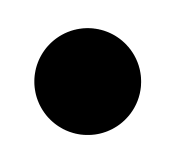
\includegraphics[scale=0.1]{../assets/0_h_tree.png}\end{tabular} & \quad & \begin{tabular}{c}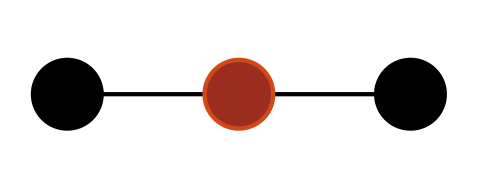
\includegraphics[scale=0.15]{../assets/h_tree_3.png}\end{tabular} & \quad & \begin{tabular}{c}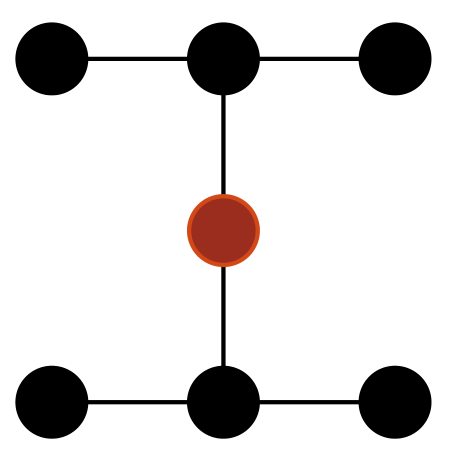
\includegraphics[scale=0.15]{../assets/h_tree_7.png}\end{tabular}
            \end{tabular}
            \caption{Cases for $h = 0$, $h = 1$ and $h = 2$.}
        \end{figure}
        Let $l_h$ and $w_h$ be the two sides of the rectangle enclosing the H tree of height $h$, respectively; thus, we have that
        
        \begin{itemize}
            \item for $h = 0$, $l_0 = w_0 = 2 \implies A_0 = l_0 \cdot w_0 = 2 \cdot 2 = 4 = 2(1+1)$ 
            \item for $h = 1$, $l_1 = 2$ and $w_1 = 4$, therefore $$A_1 = l_1 \cdot w_1 = 2 \cdot 4 = 8 = 2(3+1)$$
            \item for $h = 2$, $l_2 = w_2 = 4 \implies A_2 = l_2 \cdot w_2 = 4 \cdot 4 = 16 = 2(7+1)$
        \end{itemize}
    }{
        Assume the result is true for an H tree of height $h - 1$.
    }{
        Two different cases must be analyzed, specifically when $h$ is \tit{odd} an $h$ is \tit{even}.
        
        \begin{itemize}
            \item For the \tit{odd} case, the sides of the rectangle are defined as follows: $$\soe{l}{l_h = l_{h - 1} = 2l_{h - 2} \\ w_h = 2w_{h - 1} = 2w_{h - 2}}$$ (note that $l_{h - 1} = 2l_{h - 2}$ and $w_{h - 1} = w_{h - 2}$). Therefore
                \begin{equation*}
                    \begin{split}
                        l_h &= 2l_{h-2} \\
                            &= \ldots \\
                            &= 2^k \cdot l_{h - 2k} \quad \quad \rbk{h - 2k = 1 \implies k = \frac{h - 1}{2}} \\
                            &= 2^\frac{h - 1}{2} \cdot l_1 \\
                            &= 2^\frac{h - 1}{2} \cdot 2 \\
                            &= 2^{\frac{h - 1}{2} + 1} \\
                            &= 2^\frac{h + 1}{2}
                    \end{split}
                \end{equation*}
                and analogously
                \begin{equation*}
                    \begin{split}
                        w_h &= 2w_{h - 2} \\
                            &= \ldots \\
                            &= 2^k \cdot w_{h - 2k} \quad \quad \rbk{h - 2k = 1 \implies k = \frac{h - 1}{2}} \\
                            &= 2^\frac{h - 1}{2} \cdot w_1 \\
                            &= 2^\frac{h - 1}{2} \cdot 4 \\
                            &= 2^{\frac{h - 1}{2} + 2} \\
                            &= 2^\frac{h + 3}{2}
                    \end{split}
                \end{equation*}
                Hence, the area is
                \begin{equation*}
                    \begin{split}
                        A_h &= l_h \cdot w_h \\
                            &= 2^\frac{h + 1}{2} \cdot 2^\frac{h + 3}{2} \\
                            &= 2^\frac{2h + 4}{2} \\
                            &= 2^{h + 2} \quad \quad (h = \log (n + 1) - 1) \\
                            &= 2^{\log(n + 1) -1 +2} \\
                            &= 2^{\log(n + 1) +1} \\
                            &= 2(n + 1)
                    \end{split}
                \end{equation*}
            \item For the \tit{even} case, the sides of the rectangle are defined as follows: $$\soe{l}{l_h = 2l_{h - 1} = 2l_{h - 2} \\ w_h = w_{h - 1} = 2w_{h - 2}}$$ (note that $l_{h - 1} = l_{h - 2}$ and $w_{h - 1} = 2w_{h - 2}$) Therefore, the calculations are analogous, but $h - 2k = 0 \implies k = \dfrac{h}{2}$ which leads to $$l_h = w_h = 2^\frac{h + 2}{2}$$ (recall that $l_0 = w_0 = 2$), hence
                \begin{equation*}
                    \begin{split}
                        A_h &= l_h \cdot w_h \\
                            &= 2^\frac{h + 2}{2} \cdot 2^\frac{h + 2}{2} \\
                            &= 2^\frac{2h + 4}{2} \\
                            &= 2^{h + 2} \\
                            &= \ldots \\
                            &= 2(n + 1)
                    \end{split}
                \end{equation*}
        \end{itemize}
    }

    \printbibliography

\end{document}
